\section{Back-end}
\begin{itemize}
    \item \textbf{Architettura generale classi/funzioni PHP}: le funzioni PHP vengono richiamate mediante chiamate JavaScript/AJAX e sono inserite all'interno di file che ne portano il nome.\\
    Fanno eccezione le funzioni che hanno il compito di interrogare il database, inserite nel file \texttt{database.php}
    \item \textbf{Schema del database}: 
    	\begin{figure}[h!]
    		\centering
    		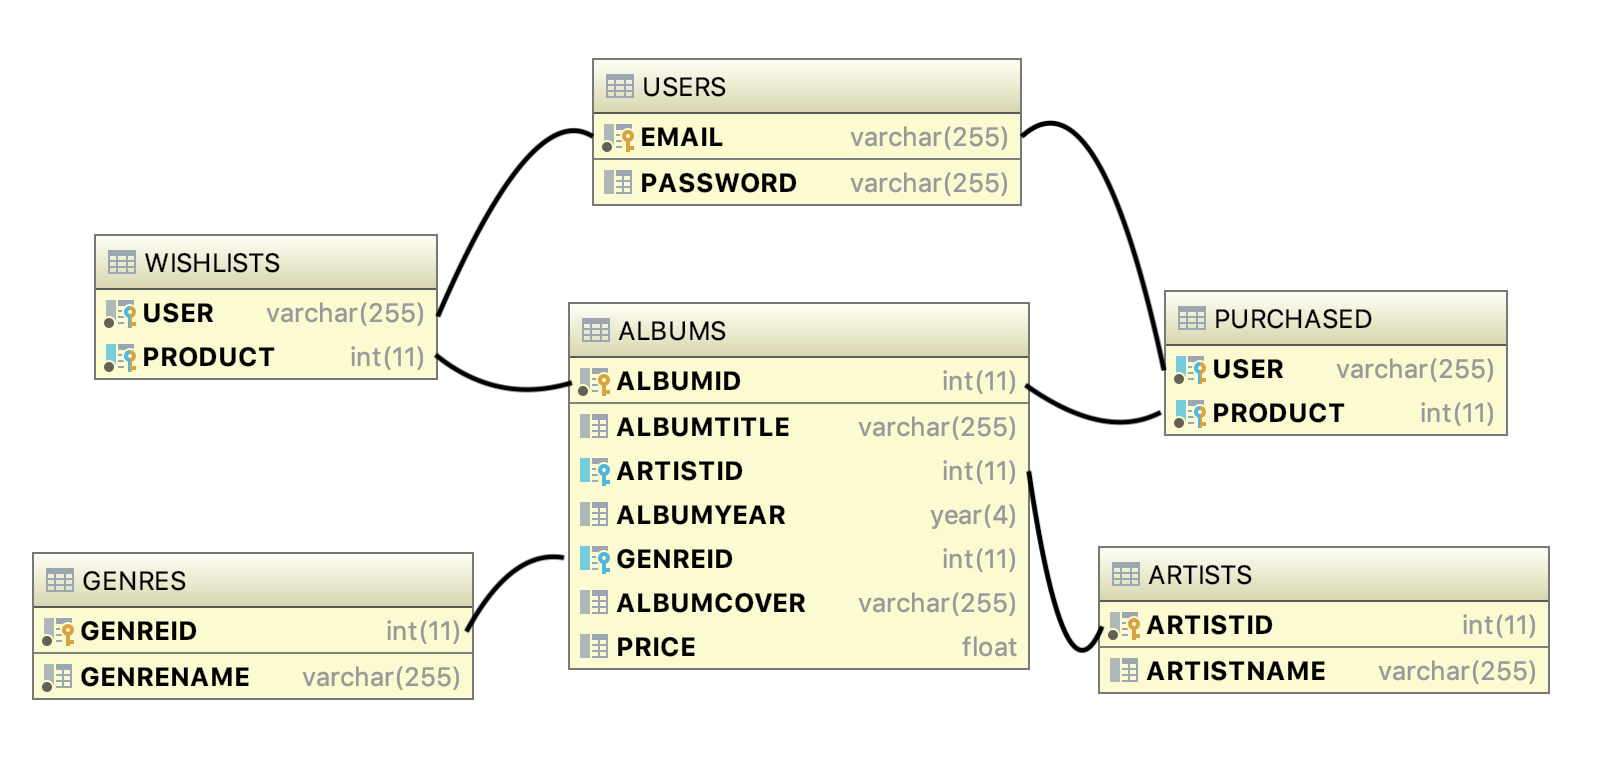
\includegraphics[scale=0.55]{schema-db.png}
    	\end{figure}
    \item \textbf{Descrizione delle funzioni remote}:
        \begin{itemize}
            \item \texttt{add\_to\_purchased.php}: viene invocata quando l'utente acquista un prodotto.\\
            Riceve in input la variabile $\texttt{\$\_POST["album"]}$, che contiene l'id dell'album da inserire tra gli acquisti e utilizza la variabile $\texttt{\$\_SESSION["user"]}$ (se questa non è impostata significa che l'utente non è loggato, quindi si viene reindirizzati alla pagina di accesso).\\
            Invia una richiesta al database che inserisce il prodotto tra gli acquistati e restituisce (in formato JSON), in caso di successo, il codice 200 alla richiesta AJAX, in caso di fallimento , il codice 404 con un messaggio di errore.
            \item \texttt{add\_to\_wishlist.php}: viene invocata quando l'utente inserisce un prodotto nella sua wishlist.\\
            Riceve in input la variabile \texttt{\$\_POST["album"]}, che contiene l'id dell'album e utilizza la variabile \texttt{\$\_SESSION["user"]} (se questa non è impostata significa che l'utente non è loggato, quindi si viene reindirizzati alla pagina di accesso).\\
            Invia una richiesta al database che inserisce il prodotto nella wishlist e restituisce (in formato JSON), in caso di successo, il codice 200, in caso di fallimento , il codice 404 con un messaggio di errore.
            \item \texttt{delete\_from\_wishlist.php}: viene invocata quando l'utente clicca sul bottone \texttt{Delete} dalla pagina che mostra la wishlist.\\
             Riceve in input la variabile \texttt{\$\_POST["album"]}, che contiene l'id dell'album e utilizza la variabile \texttt{\$\_SESSION["user"]} (se questa non è impostata significa che l'utente non è loggato, quindi si viene reindirizzati alla pagina di accesso).\\
            Invia una richiesta al database che rimuove il prodotto dalla wishlist e restituisce (in formato JSON), in caso di successo, il codice 200 e la copia della wishlist aggiornata, in caso di fallimento , il codice 404 con un messaggio di errore.
            \item \texttt{get\_album.php}: viene invocata quando l'utente clicca su un album per visualizzarne i dettagli.\\
            Riceve in input la variabile \texttt{\$\_POST["album"]}, che contiene l'id dell'album (se questa non è impostata viene restituito un messaggio di errore). 
            Il server interroga il database per ottenere tutti i dettagli sull'album (viene generato un messaggio di errore anche nel caso in cui l'album selezionato non sia presente) e restituisce le informazioni ricavate (in formato JSON) nel caso in cui la ricerca sia andata a buon fine.
            \item \texttt{get\_bestsellers.php}: questa funzione restituisce, in formato JSON, gli album più venduti presenti nel database.\\
            In caso di errore, viene generato un messaggio che informa l'utente.
            \item \texttt{get\_by\_genre.php}: riceve in input la variabile \texttt{\$\_POST["genre"]}, che contiene l'id del genere musicale selezionato dall'utente (se questa non è impostata viene restituito un messaggio di errore) e, interrogando il database, restituisce la lista degli album di tale genere in formato JSON.\\
            Nel caso in cui si verifichi un errore, viene generato un messaggio che informa l'utente.
            \item \texttt{get\_genres.php}: questa funzione restituisce una lista, in formato JSON, di tutti i generi presenti nel database. \\
            Nel caso in cui si verifichi un errore, viene generato un messaggio che informa l'utente.
            \item \texttt{get\_purchased.php}: utilizzando la variabile \texttt{\$\_SESSION["user"]}, resituisce la lista degli album acquistati dall'utente. \\
            Se la variabile \texttt{\$\_SESSION["user"]} non è impostata significa che l'utente non è loggato, quindi si viene reindirizzati alla pagina di accesso.\\
            Nel caso in cui si verifichi un errore, viene generato un messaggio che informa l'utente.
            \item \texttt{get\_wishlist.php}: utilizzando la variabile \texttt{\$\_SESSION["user"]}, resituisce la lista degli album che l'utente ha inserito nella sua wishlist. \\
            Se la variabile \texttt{\$\_SESSION["user"]} non è impostata significa che l'utente non è loggato, quindi si viene reindirizzati alla pagina di accesso.\\
            Nel caso in cui si verifichi un errore, viene generato un messaggio che informa l'utente.
            \item \texttt{login.php}: questa funzione riceve in input le variabili \texttt{\$\_POST["email"]} e \texttt{\$\_POST["password"]} e ne verifica la validità.\\
            Nel caso in cui si verifichi un errore, viene generato un messaggio che informa l'utente.
            \item \texttt{logout.php}: questa funzione riceve in input la variabile \texttt{\$\_SESSION["user"]}, distrugge le variabili di sessione e reindirizza l'utente alla pagina di accesso al sito.\\
            Nel caso in cui si verifichi un errore, viene generato un messaggio che informa l'utente.
            \item \texttt{subscribe.php}: questa funzione riceve in input le variabili \texttt{\$\_POST["email"]} e \texttt{\$\_POST["password"]}, ne verifica la validità e verifica che l'utente non sia presente nel database.\\
            Nel caso in cui si verifichi un errore, viene generato un messaggio che informa l'utente.
        \end{itemize}
    \item \textbf{Gestione delle condizioni di errore}: le condizioni di errore vengono gestite come segue:
    	\begin{itemize}
    		\item Errore nella connessione al server o nella chiamata AJAX: l'utente viene reindirizzato alla pagina di accesso al sito, dove visualizza un messaggio di errore che lo invita a riprovare.
    		\item Errore nell'input dei dati: viene visualizzato un messaggio all'interno del form che spiega l'errore commesso.
    	\end{itemize}
    \item \textbf{Funzioni di callback lato Javascript/AJAX}:
        \begin{itemize}
            \item \texttt{add\_to\_purchased}: questa funzione (richiesta di tipo \texttt{GET}) viene invocata nel momento in cui l'utente trascina la copertina dell'album da acquistare nell'apposita area, e richiede al server l'aggiunta dell'album agli acquisti.\\
            Il server risponde indicando il successo o il fallimento dell'operazione.
            \item \texttt{add\_to\_wishlist}: questa funzione (richiesta di tipo \texttt{GET}) viene invocata nel momento in cui l'utente trascina la copertina dell'album da acquistare nell'apposita area, e richiede al server l'aggiunta dell'album alla wishlist.\\
            Il server risponde indicando il successo o il fallimento dell'operazione.
            \item \texttt{delete\_from\_wishlist}: questa funzione viene invocata nel momento in cui l'utente clicca sul pulsante \texttt{Delete} di un elemento della wishlist.\\
            Viene inviata una richiesta al server (di tipo \texttt{POST}), includendo l'ID dell'album da cancellare, e il server risponde con una copia della wishlist aggiornata, che viene ricaricata su schermo.\\
            In caso di errore, l'utente viene informato con un messaggio.
            \item \texttt{get\_album}: questa funzione permette di visualizzare i dettagli di album.\\
            Viene inviata una richiesta al server (di tipo \texttt{POST}), includendo l'ID dell'album e il server risponde con le informazioni richieste.\\
            In caso di errore, l'utente viene informato con un messaggio.
            \item \texttt{get\_bestsellers}: questa funzione permette di visualizzare gli album più venduti.\\
            Viene inviata una richiesta al server (di tipo \texttt{GET}), e il server risponde (in caso di successo) con le informazioni richieste.\\
            In caso di errore, l'utente viene informato con un messaggio.
            \item \texttt{get\_by\_genre}: questa funzione permette di visualizzare tutti gli album di un dato genere.\\
            Viene inviata una richiesta al server (di tipo \texttt{POST}), inviando l'ID del genere selezionato, e il server risponde (in caso di successo) con la lista richiesta.\\
            In caso di errore, l'utente viene informato con un messaggio.
            \item \texttt{get\_genres}: questa funzione viene invocata nel momento in cui viene caricata la barra di navigazione e permette di popolare il menu dropdown con i generi presenti nel database.\\
            Si tratta di una richiesta di tipo \texttt{GET}, che restituisce la lista in caso di successo e un messaggio di errore in caso di fallimento.
            \item \texttt{get\_purchased}: questa richiesta (di tipo \texttt{GET}) riceve la lista degli album acquistati da un dato utente, in caso di successo, mentre in caso di fallimento restituisce un messaggio di errore. 
            \item \texttt{get\_wishlist}:questa richiesta (di tipo \texttt{GET}) riceve la wishlist di un dato utente, in caso di successo, mentre in caso di fallimento restituisce un messaggio di errore. 
            \item \texttt{login}: questa richiesta invia al server (mediante \texttt{POST}) l'email e la password inseriti dall'utente: in caso queste non siano valide (non esiste alcun utente con tale email o la password non è quella giusta per quell'utente), il server risponde con un messaggio di errore. Nel caso, invece, la richiesta vada a buon fine, l'utente viene reindirizzato alla home page del sito.
            \item \texttt{subscribe}: questa richiesta invia al server (mediante \texttt{POST}) l'email e la password inseriti dall'utente: in caso queste non siano valide (la password non è valida oppure esiste già un utente con tale indirizzo email), il server risponde con un messaggio di errore. Nel caso, invece, la richiesta vada a buon fine, l'utente viene reindirizzato alla home page del sito. 
        \end{itemize}
\end{itemize}